  %%%%%%%%%%%%%%%%%%%%%%%%%%%%%%%%%%%%%%%%%%%%%%%%%%%%%%%%%%%%%%%%%%%%%%
% LaTeX Example: Project Report

%%% Preamble
\documentclass[paper=a4, fontsize=11pt, abstract=on]{scrartcl}
\usepackage[T1]{fontenc}
\usepackage{fourier}
\usepackage{tabularx}
\usepackage[utf8]{inputenc}
\usepackage{hyperref}





\usepackage{listings}
\usepackage{color}

\definecolor{dkgreen}{rgb}{0,0.6,0}
\definecolor{gray}{rgb}{0.5,0.5,0.5}
\definecolor{mauve}{rgb}{0.58,0,0.82}
\lstset{frame=tb,
  language=[Visual]C++,
  aboveskip=3mm,
  belowskip=3mm,
  showstringspaces=false,
  columns=flexible,
  basicstyle={\small\ttfamily},
  numbers=none,
  numberstyle=\tiny\color{gray},
  keywordstyle=\color{blue},
  commentstyle=\color{dkgreen},
  stringstyle=\color{mauve},
  breaklines=true,
  breakatwhitespace=true,
  tabsize=3
}
\usepackage{graphicx}
\usepackage{caption}
\usepackage{subcaption}

\usepackage[english]{babel}															% English language/hyphenation
\usepackage[protrusion=true,expansion=true]{microtype}	
\usepackage{amsmath,amsfonts,amsthm} % Math packages

\usepackage{url}
%\usepackage[hang, small,labelfont=bf,up,textfont=it,up]{caption}


%%% Custom sectioning
\usepackage{sectsty}
\allsectionsfont{\normalfont\scshape}
\usepackage{float}
\usepackage{amsmath}
\usepackage{mathtools}
\usepackage{ragged2e}

\usepackage{nomencl}
\makenomenclature

%%% Custom headers/footers (fancyhdr package)
\usepackage{fancyhdr}
\pagestyle{fancyplain}
\fancyhead{}											% No page header
\fancyfoot[L]{}											% Empty 
\fancyfoot[C]{}											% Empty
\fancyfoot[R]{\thepage}									% Pagenumbering
\renewcommand{\headrulewidth}{0pt}			% Remove header underlines
\renewcommand{\footrulewidth}{0pt}				% Remove footer underlines
\setlength{\headheight}{13.6pt}
   \renewcommand*\abstractname{Summary}

%%% Equation and float numbering
\numberwithin{equation}{section}		% Equationnumbering: section.eq#
\numberwithin{figure}{section}			% Figurenumbering: section.fig#
\numberwithin{table}{section}				% Tablenumbering: section.tab#


%%% Maketitle metadata

\newcommand{\horrule}[1]{\rule{\linewidth}{#1}} 	% Horizontal rule

\title{
		%\vspace{-1in} 	
		\usefont{OT1}{bch}{b}{n}
		\normalfont \normalsize \textsc{} \\ [25pt]
		
\includegraphics[width=0.2\linewidth]{ubc.png} \\
		%
\includegraphics[width=0.4\linewidth]{tru}		
		\horrule{0.5pt} \\[0.2cm]
		\huge Term Project : Temperature Distribution inside Hydrogen Storage Tank \\
		\horrule{2pt} \\[0.005cm]
}
\author{
		\normalfont 								\normalsize
        Jerin Roberts\\[-5pt]		\normalsize
        \today
}
\date{}




%%% Begin document
\begin{document}
\maketitle
\begin{center}
\begin{tabular}{l r}


Supervisor: & Dr. Patrick Kirchen  \\ % supervisor
Locations: & University of British Columbia


\end{tabular}
\end{center}
\newpage
\begin{abstract}
  need abstract
\end{abstract}


\newpage
\tableofcontents
\listoffigures
\listoftables
\newpage
\lstset{language=[Visual]C++}

\mbox{}% need to run this: makeindex TermProject.nlo -s nomencl.ist -o TermProject.nls

 
\nomenclature{$\rho$}{Density $kg/m^3$}
\nomenclature{$C_D$}{Drag Coefficient}
\nomenclature{$C_L$}{Lift Coefficient}
\nomenclature{$C_P$}{Pressure Coefficient}
\nomenclature{$Re$}{Reynolds Number}
\nomenclature{$A$}{Cross-Sectional Projected Area $m^2$}
\nomenclature{$v$}{Velocity $m/s$}
\nomenclature{$m$}{Mass $kg$}
\nomenclature{$\mu$}{Dynamic Viscosity $Pa-s$}
\nomenclature{$L$}{Characteristic Linear Dimension $m$}
\nomenclature{$q$}{Manometer Reading $mm$}
\nomenclature{$s$}{Airfoil span $m$}
\nomenclature{$c$}{Airfoil chord $m$}
 
\printnomenclature

\newpage
\section{Introduction}


A Hydrogen has long been in consideration as of the top ecological replacements to gasoline fuelled internal combustion engines. Having a high specific energy density of 39 $kWh/kg$ and only water production as emissions hydrogen fuel could provide an effective alternative. However ghydrogen has a very low volumetric energy density 3.5 $kWh/m^3$ at standard temperatures gaseous and conditions making it difficult to store effectively and efficiently. 


%26 lines aprox 1page double spaced
\section{Background}
\subsection{Storage Sates}
The two prevailing states for storing are in compressed gaseous and cryogenic liquid states, however both methods still present a number technical challenges that need to be overcome before the technology can be successfully implemented into modern transportation infrastructures. 

At first glance the liquid form seems to be the ideal solution. Having a very high specific and volumetric energy density it can expanded into a gas easily for combustion. The two challenges that are faced with liquid hydrogen are the process for obtaining a liquid state and the measures for preserving that state. Acquiring liquid hydrogen requires various throttling and cool down methods to bring the hydrogen to a low enough temperatures to liquefy. To exist as a liquid the H2 must be cooled below hydrogen's critical point of 33 K and in order to maintain a fully liquid state without boiling at atmospheric pressure needs to be cooled further to 20.28 K. Maintaining the temperatures requires cryogenic storage technology such as thermally insulated containers and requires special handling procedures common to all cryogenic fuels. However even with thermally insulated containers it is difficult to keep such a low temperature, and the hydrogen will gradually leak away usually at a rate of about 1\% per day. These technical challenges will require additional expensive and complex systems, which makes liquid hydrogen less ideal as an energy carrier.

\begin{figure}[H]
        
        \begin{subfigure}[H]{0.45\textwidth}
        \centering
                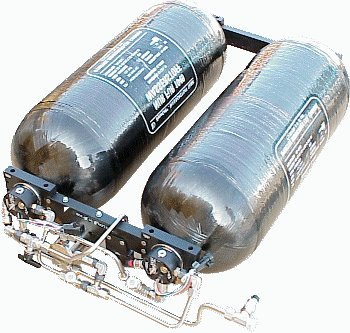
\includegraphics[height = 4.5cm]{tank1}
                \caption{}				
        \end{subfigure}%
       ~~~~~
        \begin{subfigure}[h]{0.45\textwidth}
        \centering
                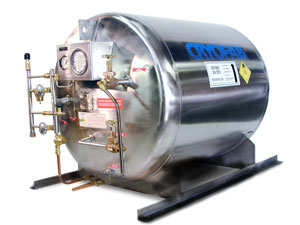
\includegraphics[height = 4.5cm]{cry}
                \caption{}
                
        \end{subfigure}
        ~~~~~
        \caption{Compressed Gaseous system (a) vs Liquid hydrogen system (b)}
        \label{results}
\end{figure}

The technical challenges of bringing compressed hydrogen fueling systems to market lie in the associated storage and re-fueling systems. Specifically using gaseous hydrogen requires significant compression of the gas in order to obtain a viable volumetric energy density +350 bar. In order to adopt these pressures while conforming to safety constraints special high pressure vessels are required.  Type 3 and 4 are typically used for high compression systems 350-700 bar. At these higher pressures the volumetric energy density of hydrogen is found to be ~1500 $kWh/m^3$, which is significantly higher than hydrogen under normal standard conditions, however still does not compare to gasoline fuels which are around 9000 $kWh/m^3$.However this is offset by hydrogen's high specific energy density and zero emissions. Another technical aspect lies in the behavior of hydrogen under fast filling conditions. In order for the technology to be successful it needs to be as good or better than current technologies. This means the refueling process needs to be as fast or faster than typical gasoline pump times. Compressing or transferring hydrogen into vehicle tanks at these pressures produces significant heat and ultimately limits the attainable fill rates. Additionally the quality of the fill is related to the temperature gain of the hydrogen during transfers. As the hydrogen cools the pressure decreases subsequently causing the tank to become partially filled.  

\subsection{Tank Types for Gaseous Hydrogen}
Pressurized Gaseous Hydrogen can be stored on board vehicles using compressed gas method. This method of storage is the simplest and most cost effective technology for hydrogen storage as it requires little supporting systems for maintenance. The gas undergoes compression at a fueling station and dispensed into the on-board tank of the vehicle. There exists 4 types of tanks used to safely store compressed hydrogen. These types are labeled as type 1,2,3 and 4. Figure \ref{tank} displays a simple diagram of a type 4 high pressure tank used for hydrogen storage.


\begin{figure}[H]
\centering
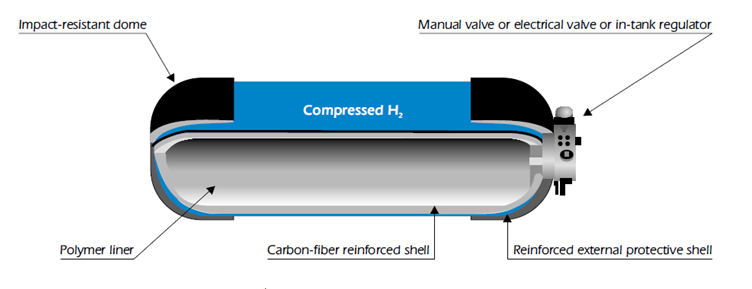
\includegraphics[width=0.8\linewidth]{tank2}
\caption{Diagram of a hydrogen  type 4 storage system}
\label{tank}
\end{figure}

 Type 1 is a basic metal tank while type is a metal tank with a fiber wrapping. These are typical of lower pressure systems (sub 300 bar) and have significantly lower performance factors due to their relatively high weight and lower capacities. Type 3 tank is a metal liner with full reinforcing fiber wrapping, while type 4 is the same as type 3 but instead with a polymer liner. These tanks are described as having a very high performance factor, attributed to their design which maximizes volume and pressure while reducing tank construction weight.  Currently, majority of demonstration and prototype vehicles employ cylinders capable of storing hydrogen up to 350 bar, while new lightweight composite type 3 and type 4 gas cylinders have been developed to withstand pressures up to 800 bar. Due to these new advances new data is required to understand the challenges with filling these tank at reasonable rates.



\subsection{Fueling}
Generally the tanks design for fuel storage will not contain any pumps or systems to maintain pressure. Therefore the hydrogen will need to be filled to rated pressure and capacity from an external source. Much like petrol stations hydrogen can be obtain through dispensers and stations in which high-pressure gas is moved from a large station reservoir into the smaller vehicle cylinder. Figure \ref{station} displays the general layout for a hydrogen dispenser. Generally the main storage tanks (supply source) will be keep the hydrogen at a lower pressure which will be compressed into buffer tanks when required. The buffer tanks allow the compressed hydrogen to remain cool and provide varying levels of pressure for efficient filling. To avoid overheating hydrogen the buffer tanks will be accessed in acceding orders of pressure. This stepping methods reduces the heat and improves efficiency of the dispenser. The rate of gas transfer and safety of filling are controlled by the station dispenser. As the temperature of the gas cools to ambient the pressure also decreases such that the cylinder is no longer filled to design capacity. This is generally termed as under filling. In order to avoid this situation cylinders are filled to rated mass, which due to the temperature increase results in the cylinder being filled beyond the rated service pressure. 

\begin{figure}[H]
\centering
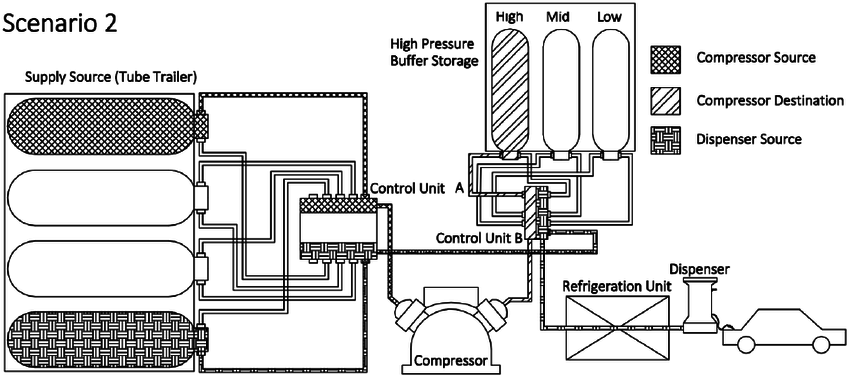
\includegraphics[width=0.8\linewidth]{station}
\caption{Simple Diagram of a hydrogen refueling station}
\label{station}
\end{figure}


 The goal of the dispenser is to fill the cylinder to the rated mass of gas without exceeding the pressure and temperature limits of the cylinder. In order to complete the filling, the dispenser must employ a method for calculating the mass of gas present inside the cylinder. Generally a flow-rate measurement and a pressure measurement will be used to estimate the total mass transferred during the fill. The metering systems for safety will need to know the values of pressure and temperature to a high accuracy and typically will have some way of receiving data from built in sensors on the vehicle tank. In order for this to be possible the temperature and pressure of the gas inside the tank need to be well characterized. With this known the location of the pressure and temperature sensors can be place appropriately as too best represent the state of the gas through out the entire tank. When the sensors are well placed they will best represent accurately the mass of hydrogen moved and allow the dispenser to know when to terminate.



\section{Theory}






\subsection{Gas Heating}
During the fill process is a significant increase in gas temperature can be seen. The temperature rise during filling is the result of the combination of two dominating phenomena; Joule-Thompson effect and standard gas compression. In thermodynamics the Joule-Thomson effect is a process in which a gas or liquid is forced through a valve or porous plug and as a result experience a temperature change. Generally most gases at room temperature cool upon expansion by the Joule-Thomson process. However a couple gases like hydrogen, helium and neon will heat when throttled. This is because their Joule-Thomson coefficient is negative corresponding to a heating effect during a free expansion. Similarly gas and liquids with positive coefficients will be cooled. It should be noted this coefficient is dependent on the state of the gas and therefore exists a point were the sign can flip which is known as the inversion temperature. Hydrogen has a negative Joule-Thomson coefficient at the temperatures and pressures of filling. Therefore when the gas experiences an isenthalpic expansion from the high-pressure tank through the dispenser throttling device into the low-pressure cylinder its temperature will increase. It is important to note that the isenthalpic expansion occurs within the dispenser which results in a higher gas temperature entering the cylinder.

\begin{equation}
\label{ideal}
PV= nRT
\end{equation}
The second phenomenon that causes a temperature rise during filling is the actual compression of the gas inside the cylinder. At the start of filling the gas is compressed by the introduction of the higher-pressure gas from the fueling station. This is repeated throughout the fill as the new gas moving into the cylinder compresses the gas currently in the cylinder. When a gas is compressed it will experience a temperature increase as is seen in equation \ref{ideal} for an ideal gas. The increase in temperature is often referred to as the heat of compression \cite{dick}. 
\begin{figure}[H]
\centering
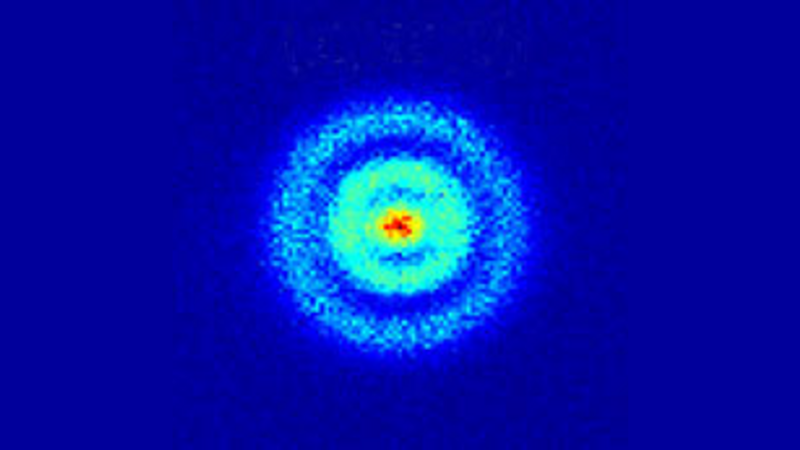
\includegraphics[width=0.8\linewidth]{hyd}
\caption{Examples of Drag coefficient as a function of Reynolds number for common objects}
\label{comp}
\end{figure}

 \begin{equation}
\label{drag}
F_D= \frac{1}{2}\rho v^2C_DA
\end{equation}


 \begin{equation}
\label{lift}
F_L= \frac{1}{2}\rho v^2C_LA
\end{equation}

\subsection{definable metrics?}


\subsection{sensor Theory}

\section{Methodology}

For this project the requirements are to map out the temperature distribution inside a hydrogen tank during a fast fill to provide a solid measure of average temperature and to find a suitable temperature location that best represents such. A combination of both modeling and experimental studies will be used to determine such point. Modeling given its valid should show the ideal location for temperature measurement. Therefore an experimental apparatus is created to help validate the thermodynamic model produced. In order to validate the model measurements of temperature at keys locations, pressure, and mass flow rate need to be recorded accurately during the entire fast fill cycle. The constraints for the experimental validation are displayed in table \ref{con}

\begin{table}[H]
\begin{center}
    \begin{tabular}{ | p{0.15\linewidth} | p{0.45\linewidth} | p{0.35\linewidth} |}
 \hline  
     \RaggedRight \textbf{Constraint}
    &\RaggedRight \textbf{Description}
    &\RaggedRight \textbf{Solution}
    \\ \hline  
           \RaggedRight 2D $\triangle T$
    &\RaggedRight Map out 2D temperature distribution within tank during transient fill
    &\RaggedRight Array of sensors with exact locations known inside tank
    \\ \hline 
           \RaggedRight $\triangle m$
    &\RaggedRight Measure accurately mass before fill, end of fill, and after cool down
    &\RaggedRight Use high accuracy scale
    \\ \hline 
           \RaggedRight $\triangle P$
    &\RaggedRight Measure Transient pressure during fast fill and cool down
    &\RaggedRight Pressure Sensor at inlet and far end of tank
    \\ \hline 
    \RaggedRight Semi-Portable
    &\RaggedRight System needs to be semi portable as system will need to be transported to hydrogen dispenser 
    &\RaggedRight Design experimental apparatus and DAQ to fit on transportable push trolley 
    \\ \hline 
    \RaggedRight Standard Tank
    &\RaggedRight No modifications to tank are permitted 
    &\RaggedRight Collapsible sensor array to be inserted and expanded inside tank
    \\ \hline 
    \RaggedRight Adhere to SAEJ2601
    &\RaggedRight Adhere to standards and procedures for the fast filling of hydrogen type 4 tanks 
    &\RaggedRight Have 1-2 sensors report data to dispenser
    \\ \hline 
    \RaggedRight Non-Invasive
    &\RaggedRight Reduce the effects of the measurement on the internal process
    &\RaggedRight Use insulating materials for sensor support, minimize size and fluid obstruction of array.
    \\ \hline 
    \end{tabular}
\end{center} 
\caption{Constraints for experimental validation}
\label{con} 
\end{table}


\subsection{Experimental Setup}
The overview of the proposed experimental setup is displayed in figure \ref{exp}
A tank will be mount to a trolley with a load cell buffer in between, which wll allow for mass change measurements. The tank will be a type 4 700 bar rated capacity tank specialized for hydrogen storage. The cylinder is manufactured by Luxfer Industries (part\# M030H) which has an internal volume that translates into 1.12 kg of stored hydrogen at a pressure of 700 bar (69.95MPa) with a temperature of 15 °C (288 K). The entire tank including fuel will weigh approximately 60 pounds. The diagram of the tank to be used in the experiment is displayed in figure \ref{tschem}. The tank contains two openings each with a 2" threaded insert. One side will be used for attaching the filling equipment while the other for the array matrix. The filling side of the cylinder will be equipped with either an off the shelf or custom internal tank valve block assembly. The assembly will house a solenoid or pneumatic valve, a manual shutoff valve, a pressure relief device, and a Bourbon reference gauge. Likely an off the shelve block will also include a thermistor mounted internally for dispenser communication. The opposite end of the cylinder will have a custom built block with support bracket for the array as well as a sealed conduit for the thermocouple wire management.


\begin{figure}[H]
\centering
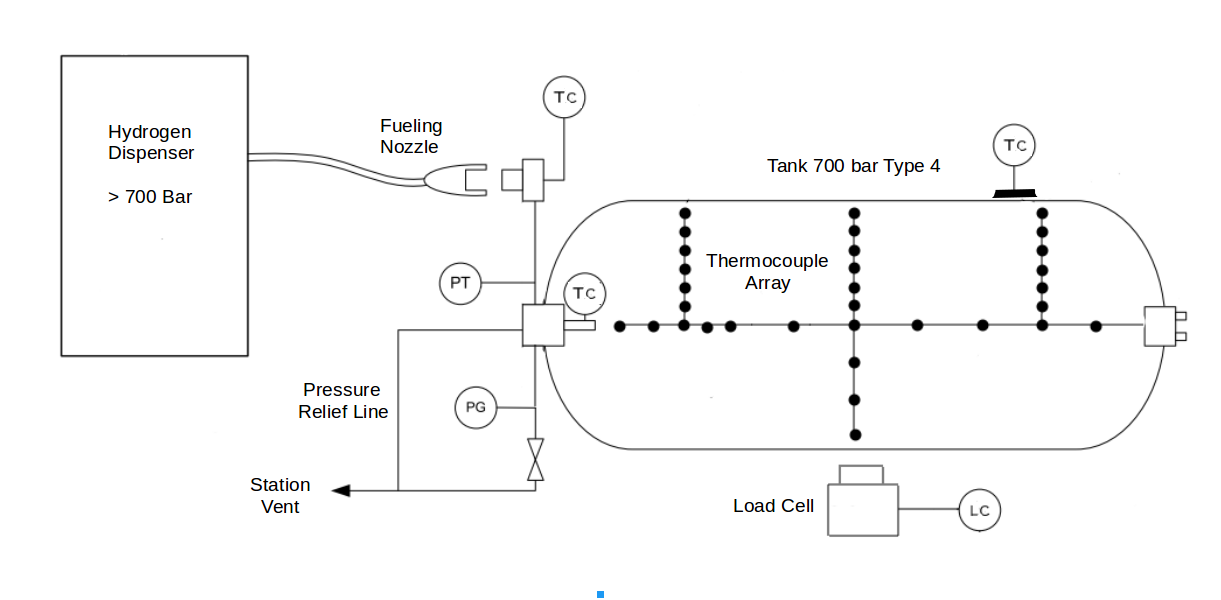
\includegraphics[width=0.95\linewidth]{schem2}
\caption{Examples of Drag coefficient as a function of Reynolds number for common objects}
\label{exp}
\end{figure}

\begin{figure}[H]
\centering
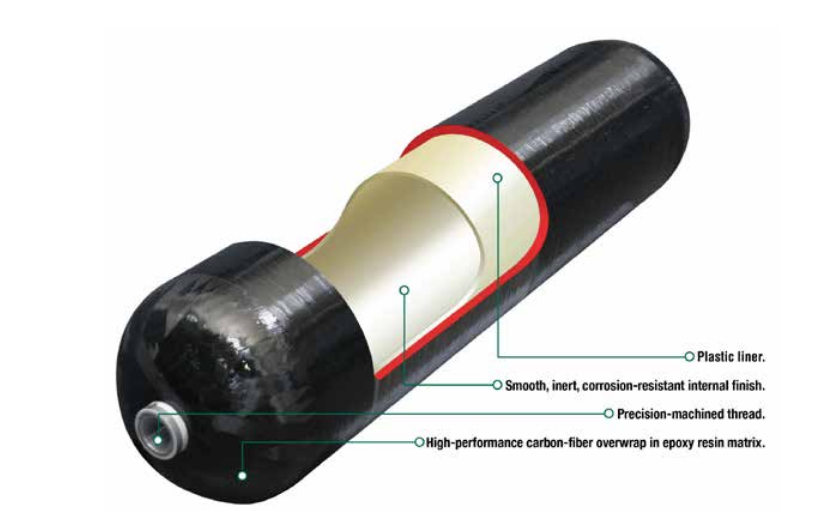
\includegraphics[width=0.95\linewidth]{tschem}
\caption{Examples of Drag coefficient as a function of Reynolds number for common objects}
\label{tschem}
\end{figure}

\subsection{DAQ} 

\subsection{Calibration}


\subsection{Procedure}


\subsection{Analysis}

 
\subsection{Uncertainty} 

\newpage 
   
\section{Results}

\subsection{Overview}


\section{Conclusion}
In this experiment we successful characterized the drag and lift coefficient for varying angles of attack. From this data a approximate stall angle was found for the Joukowski airfoil. Furthermore different methods for calculating the lift coefficient for the airfoil were investigated and found to be in poor agreement with theory and could be further improved with error mitigation or with an improved method of calibration. It was discovered that the airfoil and the plate experience the transition from viscous drag to wave drag at similar Reynolds ranges or more specifically the transition from laminar to turbulent flows. This experiment provided a great base for understanding the considerations necessary when making measurements regarding pressure, drag and lift with respect to fluid flow.





\newpage



\appendix
\section{Appendix} \label{App:Appendix}
\subsection{Joukowski Airfoil Pressure Tap}



\subsection{}




\begin{thebibliography}{99} % Beamer does not support BibTeX so references must be inserted manually as below
\bibitem[Rothuizen, 2013]{p1} Rothuizen, Erasmus Damgaard; Rokni, Masoud; Elmegaard, Brian (2013)
\newblock "A Thermodynamic Analysis of Fuelling Hydrogen Vehicles for Personal Transportation" Technical University of Denmark
\newblock Nils Koppels Allé, Bldg. 403 DK-2800 Kongens Lyngby Denmark


\bibitem[Dicken, 2006]{dick} Dicken, Chris;(2006)
\newblock "Temperature Distribution within a Compressed Gas Cylinder during Fast Filling"
\newblock  Advanced Materials Research, Vols. 15-17, pp. 281-286, 2007 


\bibitem[Hirotani et al, 2006]{p3} Hirotani, R.
Tomioka, J. ;Maeda, Y. ;Mitsuishi, H. ;Watanabe, S.;(2006)
\newblock "Thermal Behavior in Hydrogen Storage Tank for Fuel Cell Vehicle on Fast Filling"
\newblock  Proceedings of the 16th World Hydrogen Energy Conference, 13-16 June 2006, Lyon (France)


\end{thebibliography}


%%% End document
\end{document}